%\VignetteEngine{knitr::knitr}
%\VignetteIndexEntry{AmpliconBiSeq: User Guide}
%\VignettePackage{AmpliconBiSeq}
% !Rnw weave = knitr
\documentclass{article}\usepackage[]{graphicx}\usepackage[]{color}
%% maxwidth is the original width if it is less than linewidth
%% otherwise use linewidth (to make sure the graphics do not exceed the margin)
\makeatletter
\def\maxwidth{ %
  \ifdim\Gin@nat@width>\linewidth
    \linewidth
  \else
    \Gin@nat@width
  \fi
}
\makeatother

\definecolor{fgcolor}{rgb}{0.345, 0.345, 0.345}
\newcommand{\hlnum}[1]{\textcolor[rgb]{0.686,0.059,0.569}{#1}}%
\newcommand{\hlstr}[1]{\textcolor[rgb]{0.192,0.494,0.8}{#1}}%
\newcommand{\hlcom}[1]{\textcolor[rgb]{0.678,0.584,0.686}{\textit{#1}}}%
\newcommand{\hlopt}[1]{\textcolor[rgb]{0,0,0}{#1}}%
\newcommand{\hlstd}[1]{\textcolor[rgb]{0.345,0.345,0.345}{#1}}%
\newcommand{\hlkwa}[1]{\textcolor[rgb]{0.161,0.373,0.58}{\textbf{#1}}}%
\newcommand{\hlkwb}[1]{\textcolor[rgb]{0.69,0.353,0.396}{#1}}%
\newcommand{\hlkwc}[1]{\textcolor[rgb]{0.333,0.667,0.333}{#1}}%
\newcommand{\hlkwd}[1]{\textcolor[rgb]{0.737,0.353,0.396}{\textbf{#1}}}%

\usepackage{framed}
\makeatletter
\newenvironment{kframe}{%
 \def\at@end@of@kframe{}%
 \ifinner\ifhmode%
  \def\at@end@of@kframe{\end{minipage}}%
  \begin{minipage}{\columnwidth}%
 \fi\fi%
 \def\FrameCommand##1{\hskip\@totalleftmargin \hskip-\fboxsep
 \colorbox{shadecolor}{##1}\hskip-\fboxsep
     % There is no \\@totalrightmargin, so:
     \hskip-\linewidth \hskip-\@totalleftmargin \hskip\columnwidth}%
 \MakeFramed {\advance\hsize-\width
   \@totalleftmargin\z@ \linewidth\hsize
   \@setminipage}}%
 {\par\unskip\endMakeFramed%
 \at@end@of@kframe}
\makeatother

\definecolor{shadecolor}{rgb}{.97, .97, .97}
\definecolor{messagecolor}{rgb}{0, 0, 0}
\definecolor{warningcolor}{rgb}{1, 0, 1}
\definecolor{errorcolor}{rgb}{1, 0, 0}
\newenvironment{knitrout}{}{} % an empty environment to be redefined in TeX

\usepackage{alltt}
\usepackage{geometry}
\geometry{verbose,tmargin=2.5cm,bmargin=2.5cm,lmargin=2.5cm,rmargin=2.5cm}


\title{ AmpliconBiSeq: User Guide}
\IfFileExists{upquote.sty}{\usepackage{upquote}}{}

\begin{document}



\author{Altuna Akalin\\ \texttt{altuna.akalin@fmi.ch}}

\maketitle

\tableofcontents

\section{Introduction}
AmpliconBiSeq is an R package for visualization and analysis of amplicon bisulfite
sequencing experiments using high-throughput sequencing techniques. This is a targeted
version of HT bisulfite sequencing. Amplicon bisulfite sequencing provides very deep 
coverage for short regions of the genome.
 

\section{Basics}
The entry point to an AmpliconBiSeq analysis is typically a set of aligned reads. These aligned 
reads will be processed by the package and an object that contains a summary for each amplicon of each sample
will be produced. This basic object can be visualized with functions provided in the package and parts of it 
can be extracted for further analysis.

\subsection{Aligning reads}
Alignment of reads should be done by \texttt{QuasR} package. The entry point to AmpliconBiSeq
analysis will be a \texttt{qProject} object obtained from \texttt{QuasR}. Below is an example code chunk
that will achieve such alignment using \texttt{QuasR} package.
\begin{knitrout}
\definecolor{shadecolor}{rgb}{0.969, 0.969, 0.969}\color{fgcolor}\begin{kframe}
\begin{alltt}
\hlkwd{library}\hlstd{(QuasR)}
\hlcom{# make clusters, needed to run in parallel}
\hlstd{cluObj}\hlkwb{=}\hlkwd{makeCluster}\hlstd{(}\hlnum{8}\hlstd{)}
\hlcom{#change this to desired location of your alignments }
\hlstd{my.alignmentsDir}\hlkwb{=}\hlstr{"/work2/gschub/altuna/projects/AmpliconTimeCourse_cre_Feldmann/aln"}
\hlcom{#assuming text files are in your working directory}
\hlstd{proj}\hlkwb{=}
  \hlkwd{qAlign}\hlstd{(}
  \hlkwc{sampleFile}\hlstd{=}\hlstr{"~/w2/projects/AmpliconTimeCourse_cre_Feldmann/readFiles.v0.txt"}\hlstd{,}
  \hlkwc{genome}\hlstd{=}\hlstr{"BSgenome.Mmusculus.UCSC.mm9"}\hlstd{,}
  \hlkwc{auxiliaryFile}\hlstd{=}\hlstr{"/work2/gschub/Juliane/scripts/Altuna/auxFile.forQuasR.txt"}\hlstd{,}
  \hlkwc{aligner}\hlstd{=}\hlstr{"Rbowtie"}\hlstd{,}
  \hlkwc{paired}\hlstd{=}\hlstr{"fr"}\hlstd{,}
  \hlkwc{bisulfite}\hlstd{=}\hlstr{"undir"}\hlstd{,}
  \hlkwc{projectName}\hlstd{=}\hlstr{"AmpliconBiSeq"}\hlstd{,}
  \hlkwc{alignmentsDir}\hlstd{=my.alignmentsDir,}
  \hlkwc{clObj}\hlstd{=cluObj}
  \hlstd{)}
\end{alltt}
\end{kframe}
\end{knitrout}

\texttt{sampleFile} and \texttt{auxiliaryFile} are tab separated text files that
contain the sample names and read locations. For the auxiliaryFile, it contains
locations of spike-in sequences that will also be aligned against. See \texttt{?qAlign}
for more information on \texttt{sampleFile} and \texttt{auxilaryFile} requirements.


\subsection{Conversion quality check by spike-ins}
The \texttt{qProject} object that contains the aligned reads can also contain alignments for spike in sequences.
These sequences will have predefined methylation properties and bisulfite conversion efficiency can be interrogated
using those. The \texttt{spikeCheck}function provides methylation statistics for spike-ins. It plots a 
histogram or set of histograms from spike-in experiments which are helpful
to deduce conversion efficiency of the experiment.

\begin{knitrout}
\definecolor{shadecolor}{rgb}{0.969, 0.969, 0.969}\color{fgcolor}\begin{kframe}
\begin{alltt}
\hlkwd{library}\hlstd{(AmpliconBiSeq)}
\end{alltt}


{\ttfamily\noindent\itshape\color{messagecolor}{\#\# Loading required package: grid\\\#\# No methods found in "{}Rsamtools"{} for requests: readBamGappedAlignments}}\begin{alltt}
\hlkwd{spikeCheck}\hlstd{(proj,} \hlkwc{auxName} \hlstd{=} \hlstr{"T7"}\hlstd{,} \hlkwc{sampleName} \hlstd{=} \hlstr{"mock4"}\hlstd{)}
\end{alltt}
\begin{verbatim}
## Ratio of methylated Cs to Total number of Cs
## 
## T7 :  0.9822
## $T7
## [1] 0.9822
\end{verbatim}
\end{kframe}

{\centering 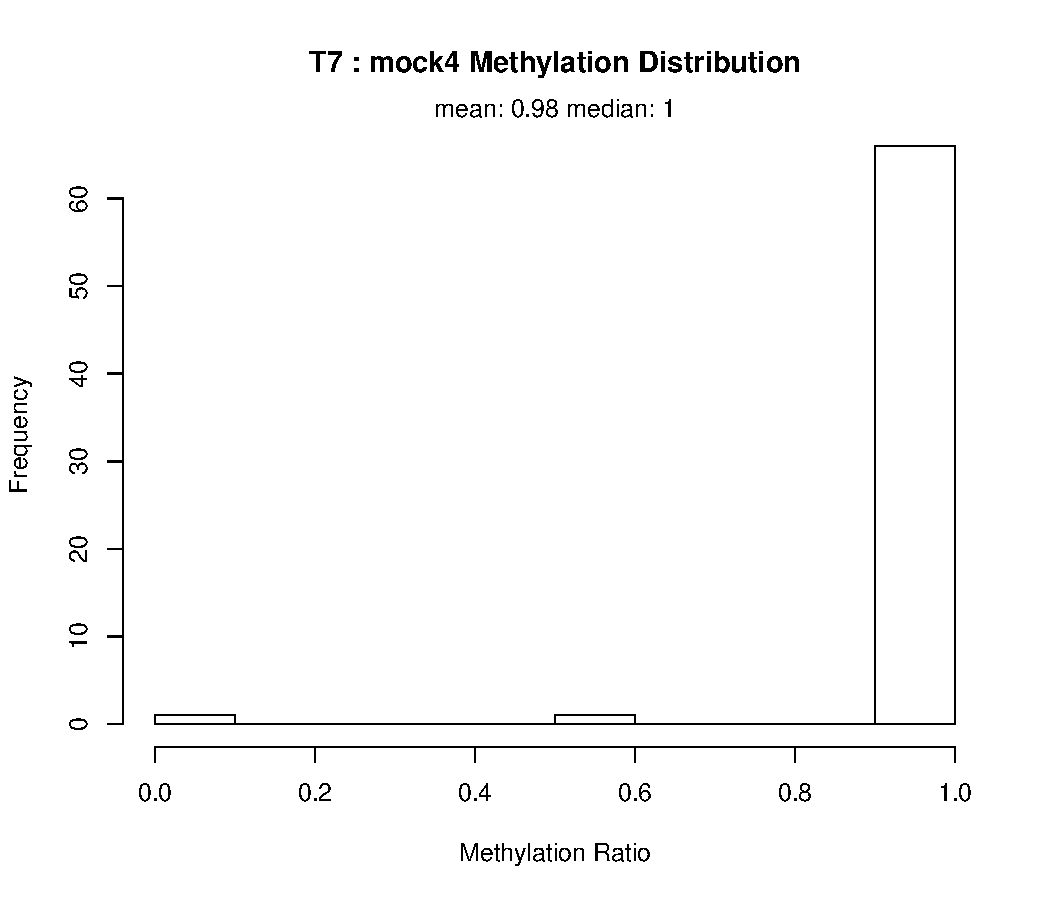
\includegraphics[width=.9\linewidth]{figure/manual-spikeCheck1} 

}



\end{knitrout}



\subsection{Extracting amplicon based methylation from alignments}
The \texttt{AmpliconViews} function extracts the amplicon related information from
the alignment and calculates meta-methylation profiles and similarity between CpGs, 
as well as average methylation values and coverage per base. The function returns
an \texttt{AmpliconViews} object. The object holds necessary information for further
analysis and visualization.

\begin{knitrout}
\definecolor{shadecolor}{rgb}{0.969, 0.969, 0.969}\color{fgcolor}\begin{kframe}
\begin{alltt}
\hlstd{ampliconLoc} \hlkwb{<-} \hlkwd{GRanges}\hlstd{(}\hlkwc{seqnames} \hlstd{=} \hlkwd{c}\hlstd{(}\hlstr{"chr18"}\hlstd{,} \hlstr{"chr18"}\hlstd{),}
    \hlkwc{ranges} \hlstd{=} \hlkwd{IRanges}\hlstd{(}\hlkwd{c}\hlstd{(}\hlnum{69674375}\hlstd{,} \hlnum{69674975}\hlstd{),} \hlkwd{c}\hlstd{(}\hlnum{69674775}\hlstd{,}
        \hlnum{69675375}\hlstd{)))}
\hlstd{x} \hlkwb{<-} \hlkwd{AmpliconViews}\hlstd{(proj,} \hlkwc{range} \hlstd{= ampliconLoc,} \hlkwc{tag} \hlstd{=} \hlkwd{c}\hlstd{(}\hlstr{"amp1"}\hlstd{,}
    \hlstr{"amp2"}\hlstd{),} \hlkwc{sampleNames} \hlstd{=} \hlkwd{c}\hlstd{(}\hlstr{"mock4"}\hlstd{),} \hlkwc{call.matrix} \hlstd{=} \hlnum{FALSE}\hlstd{,}
    \hlkwc{verbose} \hlstd{=} \hlnum{TRUE}\hlstd{)}
\hlstd{x}
\end{alltt}
\end{kframe}
\end{knitrout}


\subsection{Visualizing Amplicons}
Amplicons can be visualized with \texttt{plotAmpliconView} function. The function
can visualize one amplicon at a time, so it is important that users select which 
amplicon they want to visualize before hand. This can be done with \texttt{getAmplicon} function.
An example of this is shown below.
\begin{knitrout}
\definecolor{shadecolor}{rgb}{0.969, 0.969, 0.969}\color{fgcolor}\begin{kframe}
\begin{alltt}
\hlkwd{data}\hlstd{(ampViewEx)}  \hlcom{# load example data}
\hlstd{myAmp} \hlkwb{<-} \hlkwd{getAmplicon}\hlstd{(ampViewEx,} \hlstr{"mock4"}\hlstd{,} \hlstr{"chr18_69674375_69674775"}\hlstd{)}
\hlkwd{plotAmpliconView}\hlstd{(myAmp)}
\end{alltt}
\end{kframe}

{\centering 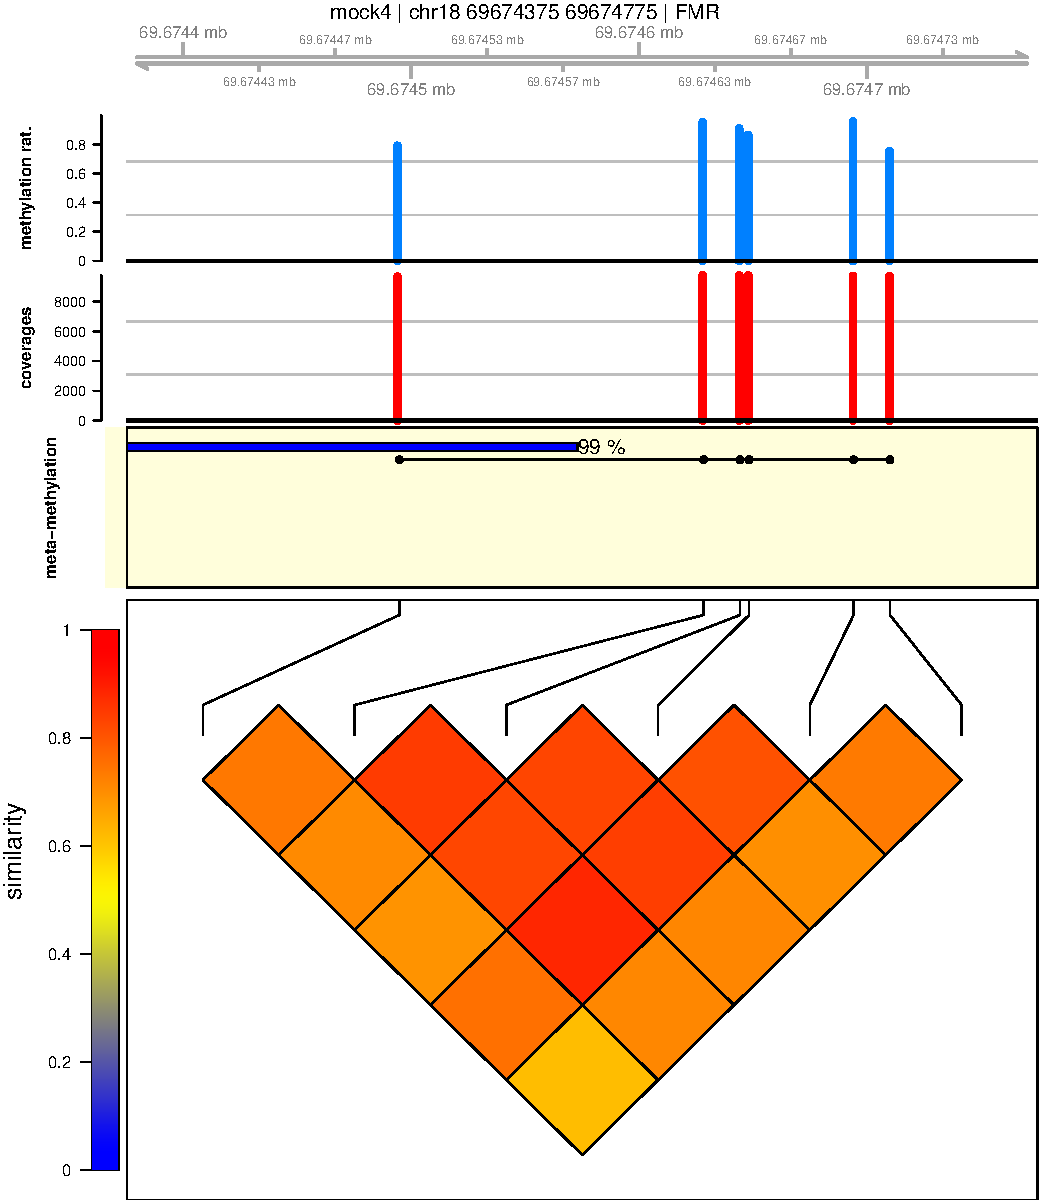
\includegraphics[width=.9\linewidth]{figure/manual-plotAmp} 

}



\end{knitrout}


\section{Calculation of meta-methylation profiles}
An amplicon can be represented as a binary methylation
call matrix where each row is a read fragment and the columns are CpGs.
Meta-methylation profiles can be thought of as patterns that explain a sub-section of 
methylation call matrix from an amplicon.  This matrix can be
analyzed to get methylation profiles that explains most of the individual profiles. This
way, huge matrices can be efficiently visualized and summarized, and this could also be
used as a metric for sample heterogeneity.
Meta-methylation profiles are calculated 
using two rounds of singular-value decomposition (different way of doing PCA) and clustering. 
First round of SVD removes the noise
using a user defined cutoff or an 'automatic' cutoff. The cutoff designates what percentage
of variation is considered as noise. The first round will basically remove principal components
that does not explain much of the variation. The second round of SVD will be run on noise
filtered matrix of methylation calls, and rows of the matrix will be clustered based
on the top contributing components (the components that explain most variation),
then for each cluster a meta-methylation profile is calculated by taking the average of 
methylation scores and binarizing them. The size of the cluster can be used
to calculate what percentage of the data has driven the given meta-methylation profile.
\\ 
In the example below, we will simulate a methylation call matrix which has three methylation
profiles and some noise. Here are the methylation profiles:
\begin{knitrout}
\definecolor{shadecolor}{rgb}{0.969, 0.969, 0.969}\color{fgcolor}

{\centering 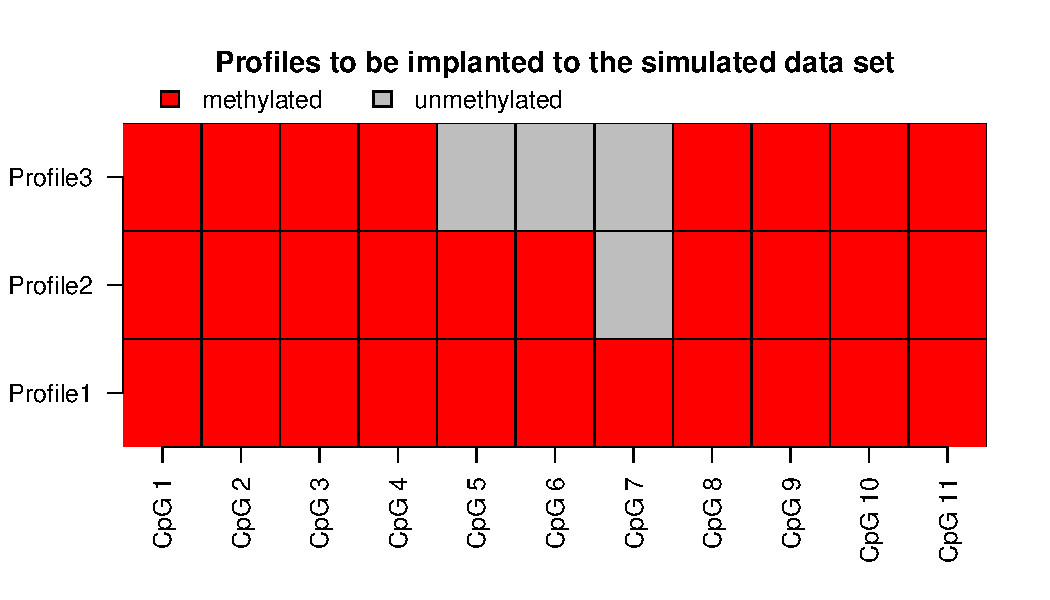
\includegraphics[width=.9\linewidth]{figure/manual-metaImplant} 

}



\end{knitrout}


Now, we will construct a simulated methylation call matrix and add some noise. "Profile1" will
be replicated 500 times, "Profile2" will be replicated 300 times and "Profile3" will
be replicated 200 times. Then we will add 5 \% noise which will represent methylation
call error or other noise.

\begin{knitrout}
\definecolor{shadecolor}{rgb}{0.969, 0.969, 0.969}\color{fgcolor}

{\centering 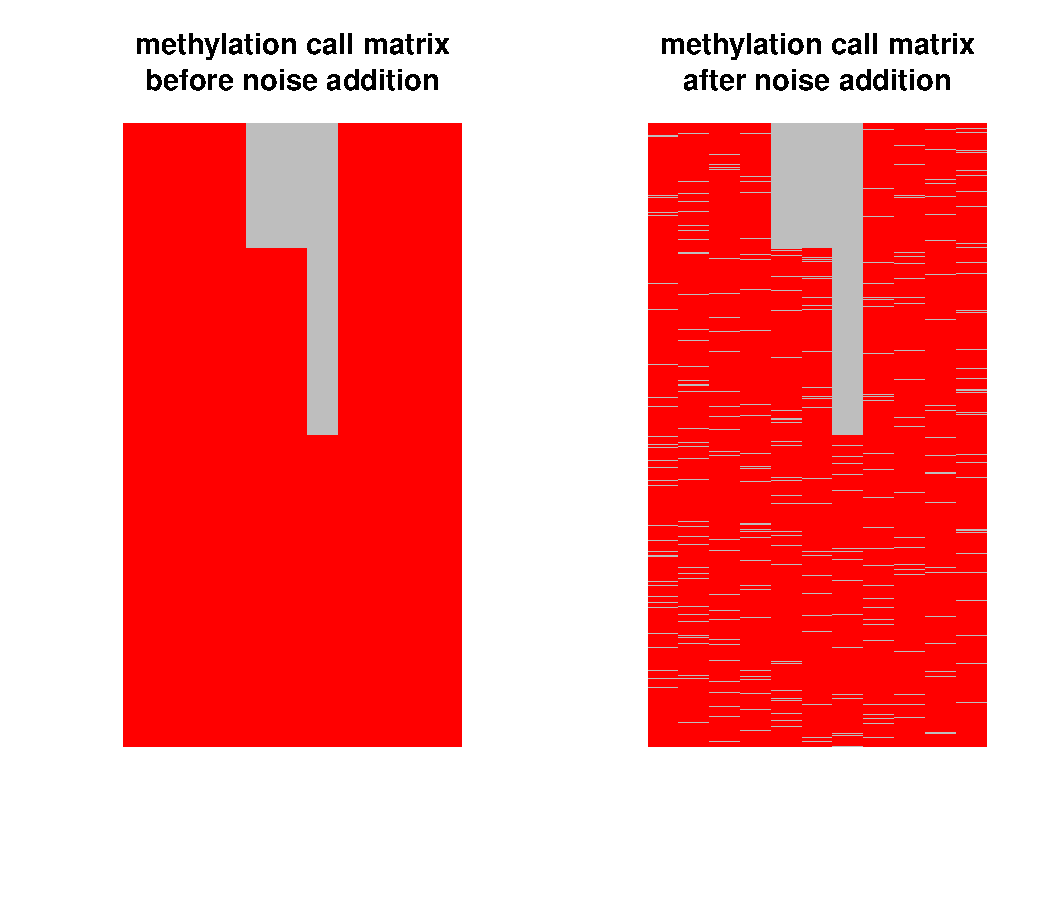
\includegraphics[width=.9\linewidth]{figure/manual-MetaGenerate} 

}



\end{knitrout}

Here are the returned meta-methylation profiles after analyzing the simulated
call matrix with the method explained above. The method also orders the meta-methylation
profiles based on how much of the data set they explain. In this example,
"Meta1" returned as most important since it, explains 44\% of the dataset. The method
returned all the implanted profiles correctly and ordered them correctly based on
how much of the data they can explain.

\begin{knitrout}
\definecolor{shadecolor}{rgb}{0.969, 0.969, 0.969}\color{fgcolor}

{\centering 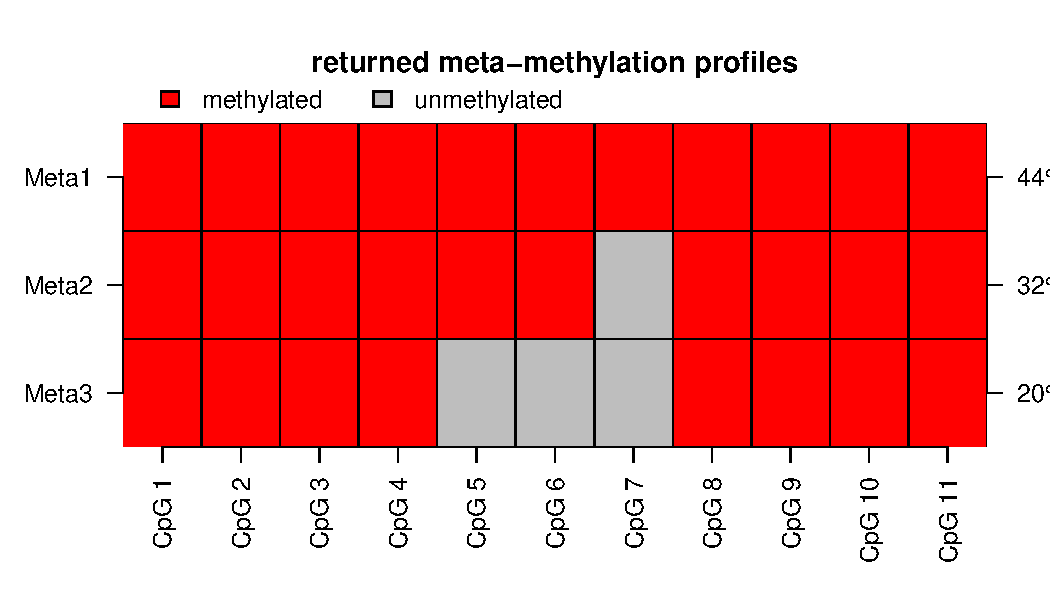
\includegraphics[width=.9\linewidth]{figure/manual-metaReveal} 

}



\end{knitrout}



\section{Calculation of similarity between CpG pairs from the same amplicon}
For a given amplicon, a similarity between a pair of CpGs can be calculated as
simple Jaccard similarity, which is number of common methylation calls over all
methylation calls for a pair of CpGs.

\begin{equation}\label{Jaccard}
 Jaccard Similarity =\frac{M_1 \cap M_2}{M_1 \cup M_2}
\end{equation}

In equation (\ref{Jaccard}), $M_1$ $\cap$ $M_2$ is the number of identical 
methylation calls for $CpG_1$ and $CpG_2$, and $M_1$ $\cup$ $M_2$ is the number
of methylation calls that are present both CpGs. For example, the Jaccard similarty between
these two binary vectors, A=[1,1,1,0,0] and B=[1,1,0,0,0] is 0.8 since 4 out 5 elements are
identical.
\\ 

There are two other experimental similarity measures calculated. One is a method suggested by Landan et. al  (doi:10.1038/ng.2442, Nature Genetics).
The other one is still the Jaccard similarity but calculated after removing data 
points where both CpGs are unmethylated. 

\section{Convenience functions}
These functions help query and extract parts of AmpliconViews object, so those parts can
be utilized in further analysis.

\subsection{Getting methylation ratio for all bases covered in experiments}
\texttt{methRatio} function can be used to get a table of methylation ratios and
coverage per base or per amplicon.
\begin{knitrout}
\definecolor{shadecolor}{rgb}{0.969, 0.969, 0.969}\color{fgcolor}\begin{kframe}
\begin{alltt}
\hlkwd{data}\hlstd{(ampViewEx)}
\hlkwd{methRatio}\hlstd{(ampViewEx)}
\end{alltt}
\begin{verbatim}
## GRanges with 546 ranges and 5 metadata columns:
##         seqnames                 ranges strand
##            <Rle>              <IRanges>  <Rle>
##     [1]    chr18   [25826977, 25826977]      *
##     [2]    chr18   [25827148, 25827148]      *
##     [3]    chr18   [69674494, 69674494]      *
##     [4]    chr18   [69674628, 69674628]      *
##     [5]    chr18   [69674644, 69674644]      *
##     ...      ...                    ...    ...
##   [542]     chr8 [114652776, 114652776]      *
##   [543]     chr8 [114652802, 114652802]      *
##   [544]     chr8 [114652823, 114652823]      *
##   [545]     chr8 [114652854, 114652854]      *
##   [546]     chr8 [114652905, 114652905]      *
##           | mock4.coverage mock4.methRatio
##           |      <numeric>       <numeric>
##     [1]   |           3683         0.02851
##     [2]   |           3694         0.03790
##     [3]   |           9669         0.79150
##     [4]   |           9772         0.95405
##     [5]   |           9765         0.91091
##     ... ...            ...             ...
##   [542]   |           3165        0.010427
##   [543]   |         124834        0.095847
##   [544]   |         124744        0.133153
##   [545]   |         124405        0.078759
##   [546]   |         123559        0.001554
##         cre10.coverage cre10.methRatio
##              <numeric>       <numeric>
##     [1]           8789         0.01422
##     [2]           8799         0.02193
##     [3]           1776         0.64640
##     [4]           1798         0.60623
##     [5]           1786         0.50280
##     ...            ...             ...
##   [542]           1541        0.041531
##   [543]         107710        0.050515
##   [544]         107666        0.047183
##   [545]         107508        0.019226
##   [546]         106984        0.004225
##                           tag
##                      <factor>
##     [1] Constitutive_LMR-REST
##     [2] Constitutive_LMR-REST
##     [3]                   FMR
##     [4]                   FMR
##     [5]                   FMR
##     ...                   ...
##   [542] Constitutive_LMR-REST
##   [543] Constitutive_LMR-REST
##   [544] Constitutive_LMR-REST
##   [545] Constitutive_LMR-REST
##   [546] Constitutive_LMR-REST
##   ---
##   seqlengths:
##     chr1 chr10 chr11 chr12 ...  chr8  chr9  chrX
##       NA    NA    NA    NA ...    NA    NA    NA
\end{verbatim}
\end{kframe}
\end{knitrout}

\subsection{Subsetting AmpliconViews}
\texttt{getAmplicon} is the function for subsetting an AmpliconViews object.
\begin{knitrout}
\definecolor{shadecolor}{rgb}{0.969, 0.969, 0.969}\color{fgcolor}\begin{kframe}
\begin{alltt}
\hlkwd{data}\hlstd{(ampViewEx)}
\hlstd{myAmp} \hlkwb{<-} \hlkwd{getAmplicon}\hlstd{(ampViewEx,} \hlkwc{sampleNames} \hlstd{=} \hlstr{"mock4"}\hlstd{,}
    \hlkwc{ampliconNames} \hlstd{=} \hlstr{"chr18_69674375_69674775"}\hlstd{)}
\end{alltt}
\end{kframe}
\end{knitrout}


\subsection{Getting amplicon and sample information}
\texttt{getAmpliconNames},\texttt{getSampleNames} are the functions that retrieve
amplicon names and sample names. \texttt{getAmpliconRanges} returns \texttt{GRanges}
object that contains the locations of the amplicons.
\begin{knitrout}
\definecolor{shadecolor}{rgb}{0.969, 0.969, 0.969}\color{fgcolor}\begin{kframe}
\begin{alltt}
\hlkwd{data}\hlstd{(ampViewEx)}
\hlstd{x} \hlkwb{<-} \hlkwd{getAmpliconNames}\hlstd{(ampViewEx)}
\hlkwd{head}\hlstd{(x)}
\end{alltt}
\begin{verbatim}
## [1] "chr18_69674375_69674775"  
## [2] "chr18_69674975_69675375"  
## [3] "chr18_69675575_69675975"  
## [4] "chr6_113705515_113705915" 
## [5] "chr11_68768916_68769316"  
## [6] "chr12_112491293_112491693"
\end{verbatim}
\begin{alltt}
\hlkwd{getSampleNames}\hlstd{(ampViewEx)}
\end{alltt}
\begin{verbatim}
## [1] "mock4" "cre10"
\end{verbatim}
\end{kframe}
\end{knitrout}

\subsection{Other functions}
There are a number of other convenience functions to access particular parts of the
\texttt{AmpliconViews} object. \texttt{getAvMeth} and \texttt{getCoverage} gets
methylation per base and coverage per base for a specific amplicon. \texttt{getExampleMethMat}
returns a sample of methylation call matrix (if there was enough coverage) on the amplicon.
\texttt{getMethMat} returns full methylation call matrix for a given amplicon, if
it was extracted during object creation.

\section{Future Work}
The package will support visualization of extra tracks \texttt{plotAmpliconView} function.



\end{document}
